\documentclass[11pt]{article}

\usepackage{graphicx}
\usepackage[margin=1in]{geometry}
\usepackage{fancyhdr}
\usepackage[brazilian]{babel}
\usepackage[utf8]{inputenc}
\usepackage[T1]{fontenc}
\usepackage{url}
\usepackage{cite}
\usepackage{indentfirst}
\usepackage{ragged2e}
\usepackage{float}
\setlength\RaggedRightParindent{15pt}

\setlength\parindent{24pt}
\setlength{\parskip}{5pt plus 1pt}
\setlength{\headheight}{13.6pt}

\newcommand\question[2]{\vspace{.25in}\hrule\textbf{#1: #2}\vspace{.5em}\hrule\vspace{.10in}}
\renewcommand\part[1]{\vspace{.10in}\textbf{(#1)}}
\newcommand\algorithm{\vspace{.10in}\textbf{Algorithm: }}
\newcommand\descricao{\vspace{.10in}\textbf{Descrição do projeto }}
\newcommand\diagrama{\vspace{.10in}\textbf{Diagrama de blocos }}
\newcommand\componentes{\vspace{.10in}\textbf{Tecnologias utilizadas}}
\newcommand\gargalos{\vspace{.10in}\textbf{Possíveis gargalos}}
\newcommand\analise{\vspace{.10in}\textbf{Analise o texto a seguir extraído do livro : “Introduction to Embedded Systems - A CyberPhysical Systems Approach (7.2.1)” e faça uma resenha sobre paralelismo e concorrência}}
\pagestyle{fancyplain}
\lhead{\textbf{\NAME\ }}
\chead{\textbf{Ideias para o projeto}}
\rhead{\today}


\begin{document}\raggedright
%Section A==============Change the values below to match your information==================
\newcommand\NAME{Marcelo G de Andrade}  % your name
\newcommand\HWNUM{1}              % the homework number
%Section B==============Put your answers to the questions below here=======================

% no need to restate the problem --- the graders know which problem is which,
% but replacing "The First Problem" with a short phrase will help you remember
% which problem this is when you read over your homeworks to study.

\question{1}{Detector de mentira}

\part{1} \descricao


\RaggedRight Esse projeto consiste em um sistema embarcado que tenha uma conexão aos dedos de uma pessoa, e como é explicado em \cite{eletrodermal}, segundo a teoria da atividade eletrodermal, a condutividade elétrica da pele humana varia de acordo com diversos aspectos psicológicos, como o estresse, assim sendo possível relacionar a condutividade elétrica da pele com o fato de uma pessoa estar mentindo ou não. O processamento desse 
sinal seria feito no microcontrolador, retornando o resultado em um display ou apenas LEDs verdes e vermelhos.

\raggedright
\part{2} \diagrama

\begin{figure}[h!]
	\centering
	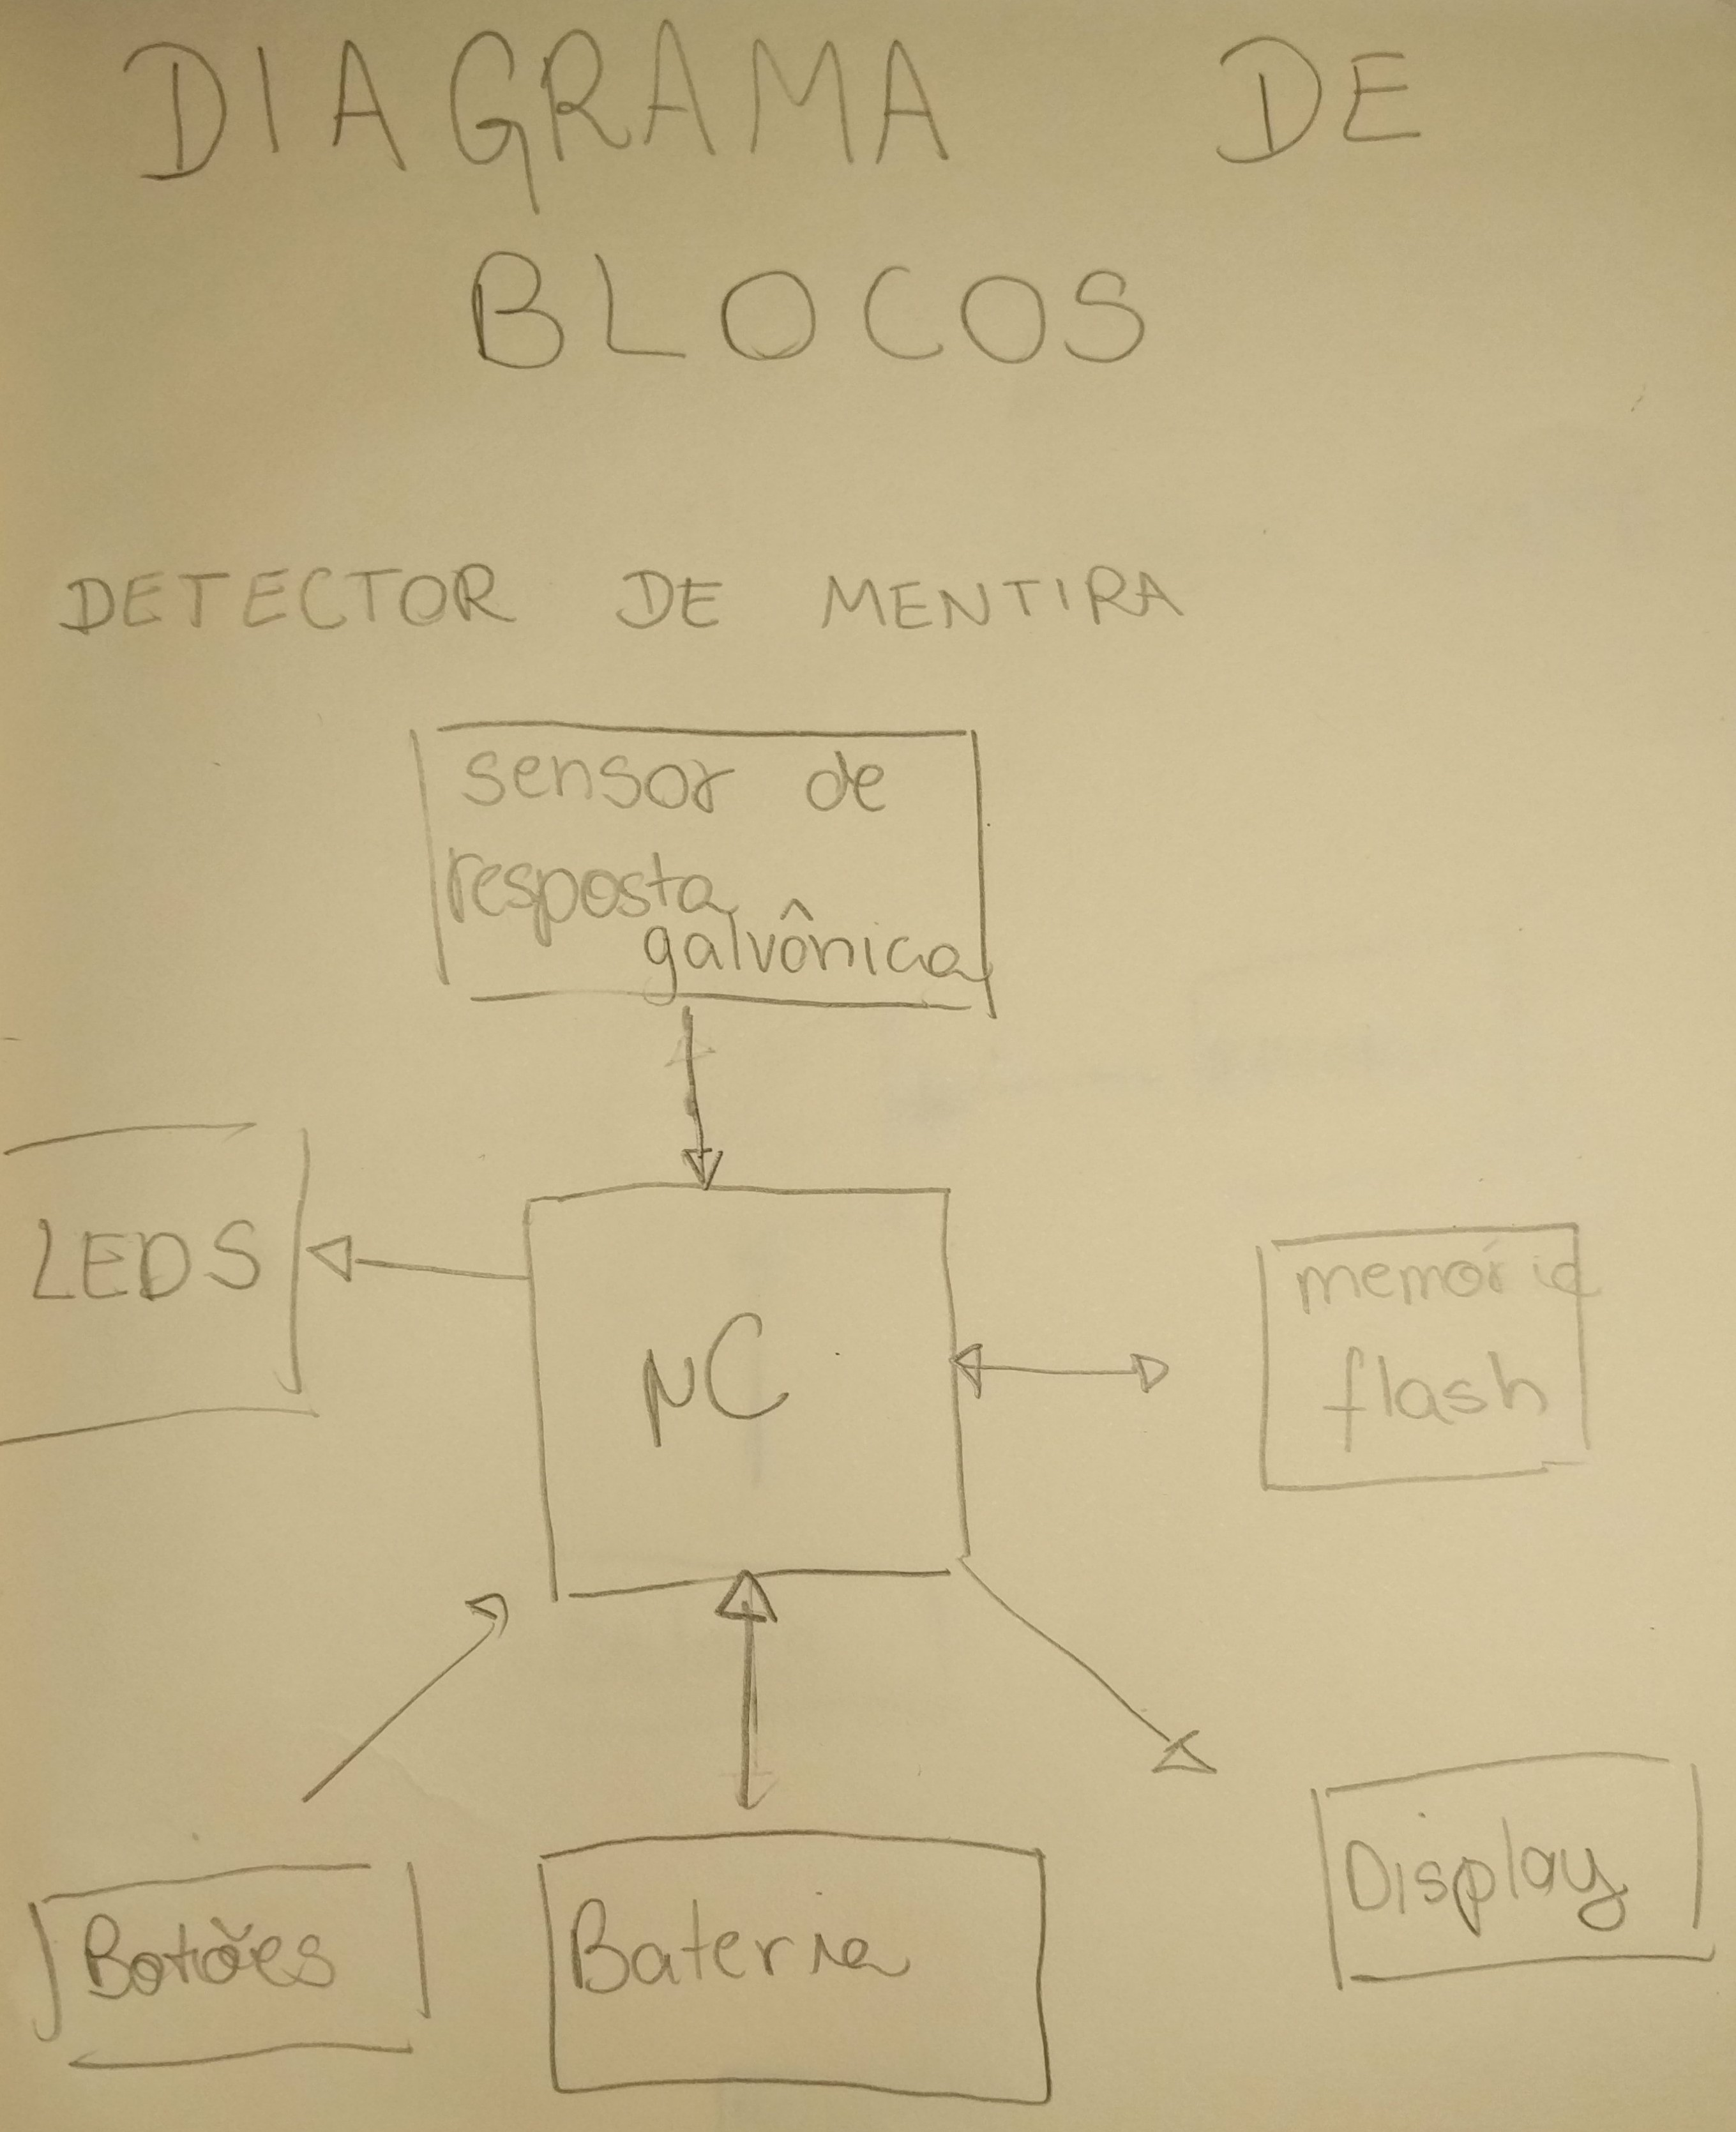
\includegraphics[width=0.7\textwidth]{fig1.jpg}
		\caption{Diagrama de blocos.}
\end{figure}

\raggedright
\part{3} \componentes

\RaggedRight O principal componente desse projeto é o sensor de resposta galvânica, capaz de medir a 
condutividade elétrica da pele com precisão. Há outros periféricos mais comuns como uma memória flash, uma bateria, LEDs ou um display, e botões para sincronizar a entrada do sistema. 

Em \cite{gsr_sensor} é vendido um sensor de média qualidade por um preço baixo, mas apenas nos Estados Unidos.

Uma alternativa para o sensor de resposta galvânica seriam os sensores biomédicos da SparksFun, como pode ser visto em \cite{biomedic_sensor}.No entanto, seria necessário estudar como pode-se relacionar as atividades neurológicas com o ato de mentir.

Na parte de software, é necessário um estudo e análise dos dados coletados. Cada pessoa tem uma resposta diferente ao sensor, portanto o mesmo deve ser calibrado cada vez que é utilizado. Para uma resposta mais precisa, seria ótimo uma análise estatística por trás do sistema, mas quanto maior a complexidade da análise, mais complicado é a implementação da mesma no processador do embarcado. Uma solução para esse problema, caso a análise seja muito avançada, é fazê-la em um servidor externo e usar o embarcado para mandar e receber os dados.


\raggedright
\part{4} \gargalos

\RaggedRight Há dois principais gargalos nesse projeto. O primeiro deles é a precisão e análise dos dados coletados pelo sensor. É preciso fazer um estudo de comportamento para tirar conclusões a respeito da condutividade elétrica da pele, o valor bruto não é suficiente para uma conclusão.

O segundo gargalo é o preço do sensor de resposta galvânica. Um sensor decente no exterior já tem um preço relativamente alto, já no Brasil, esse preço é muito mais alto e a os sensores são extremamente raros.


\raggedright
\question{2}{Carro controlado pela mente}

\part{1} \descricao


\RaggedRight Esse projeto consiste de um simples carrinho com movimentações limitadas (frente e trás). Os movimentos desse carrinho seriam mandados através de ondas eletromagnéticas geradas pelo dispositivo embarcado. Esses sinais seriam gerados a partir de um sensor biomédico de atividade neurológica, como pode ser visto em \cite{biomedic_sensor}. 

\raggedright
\part{2} \diagrama

\begin{figure}[H]
	\centering
	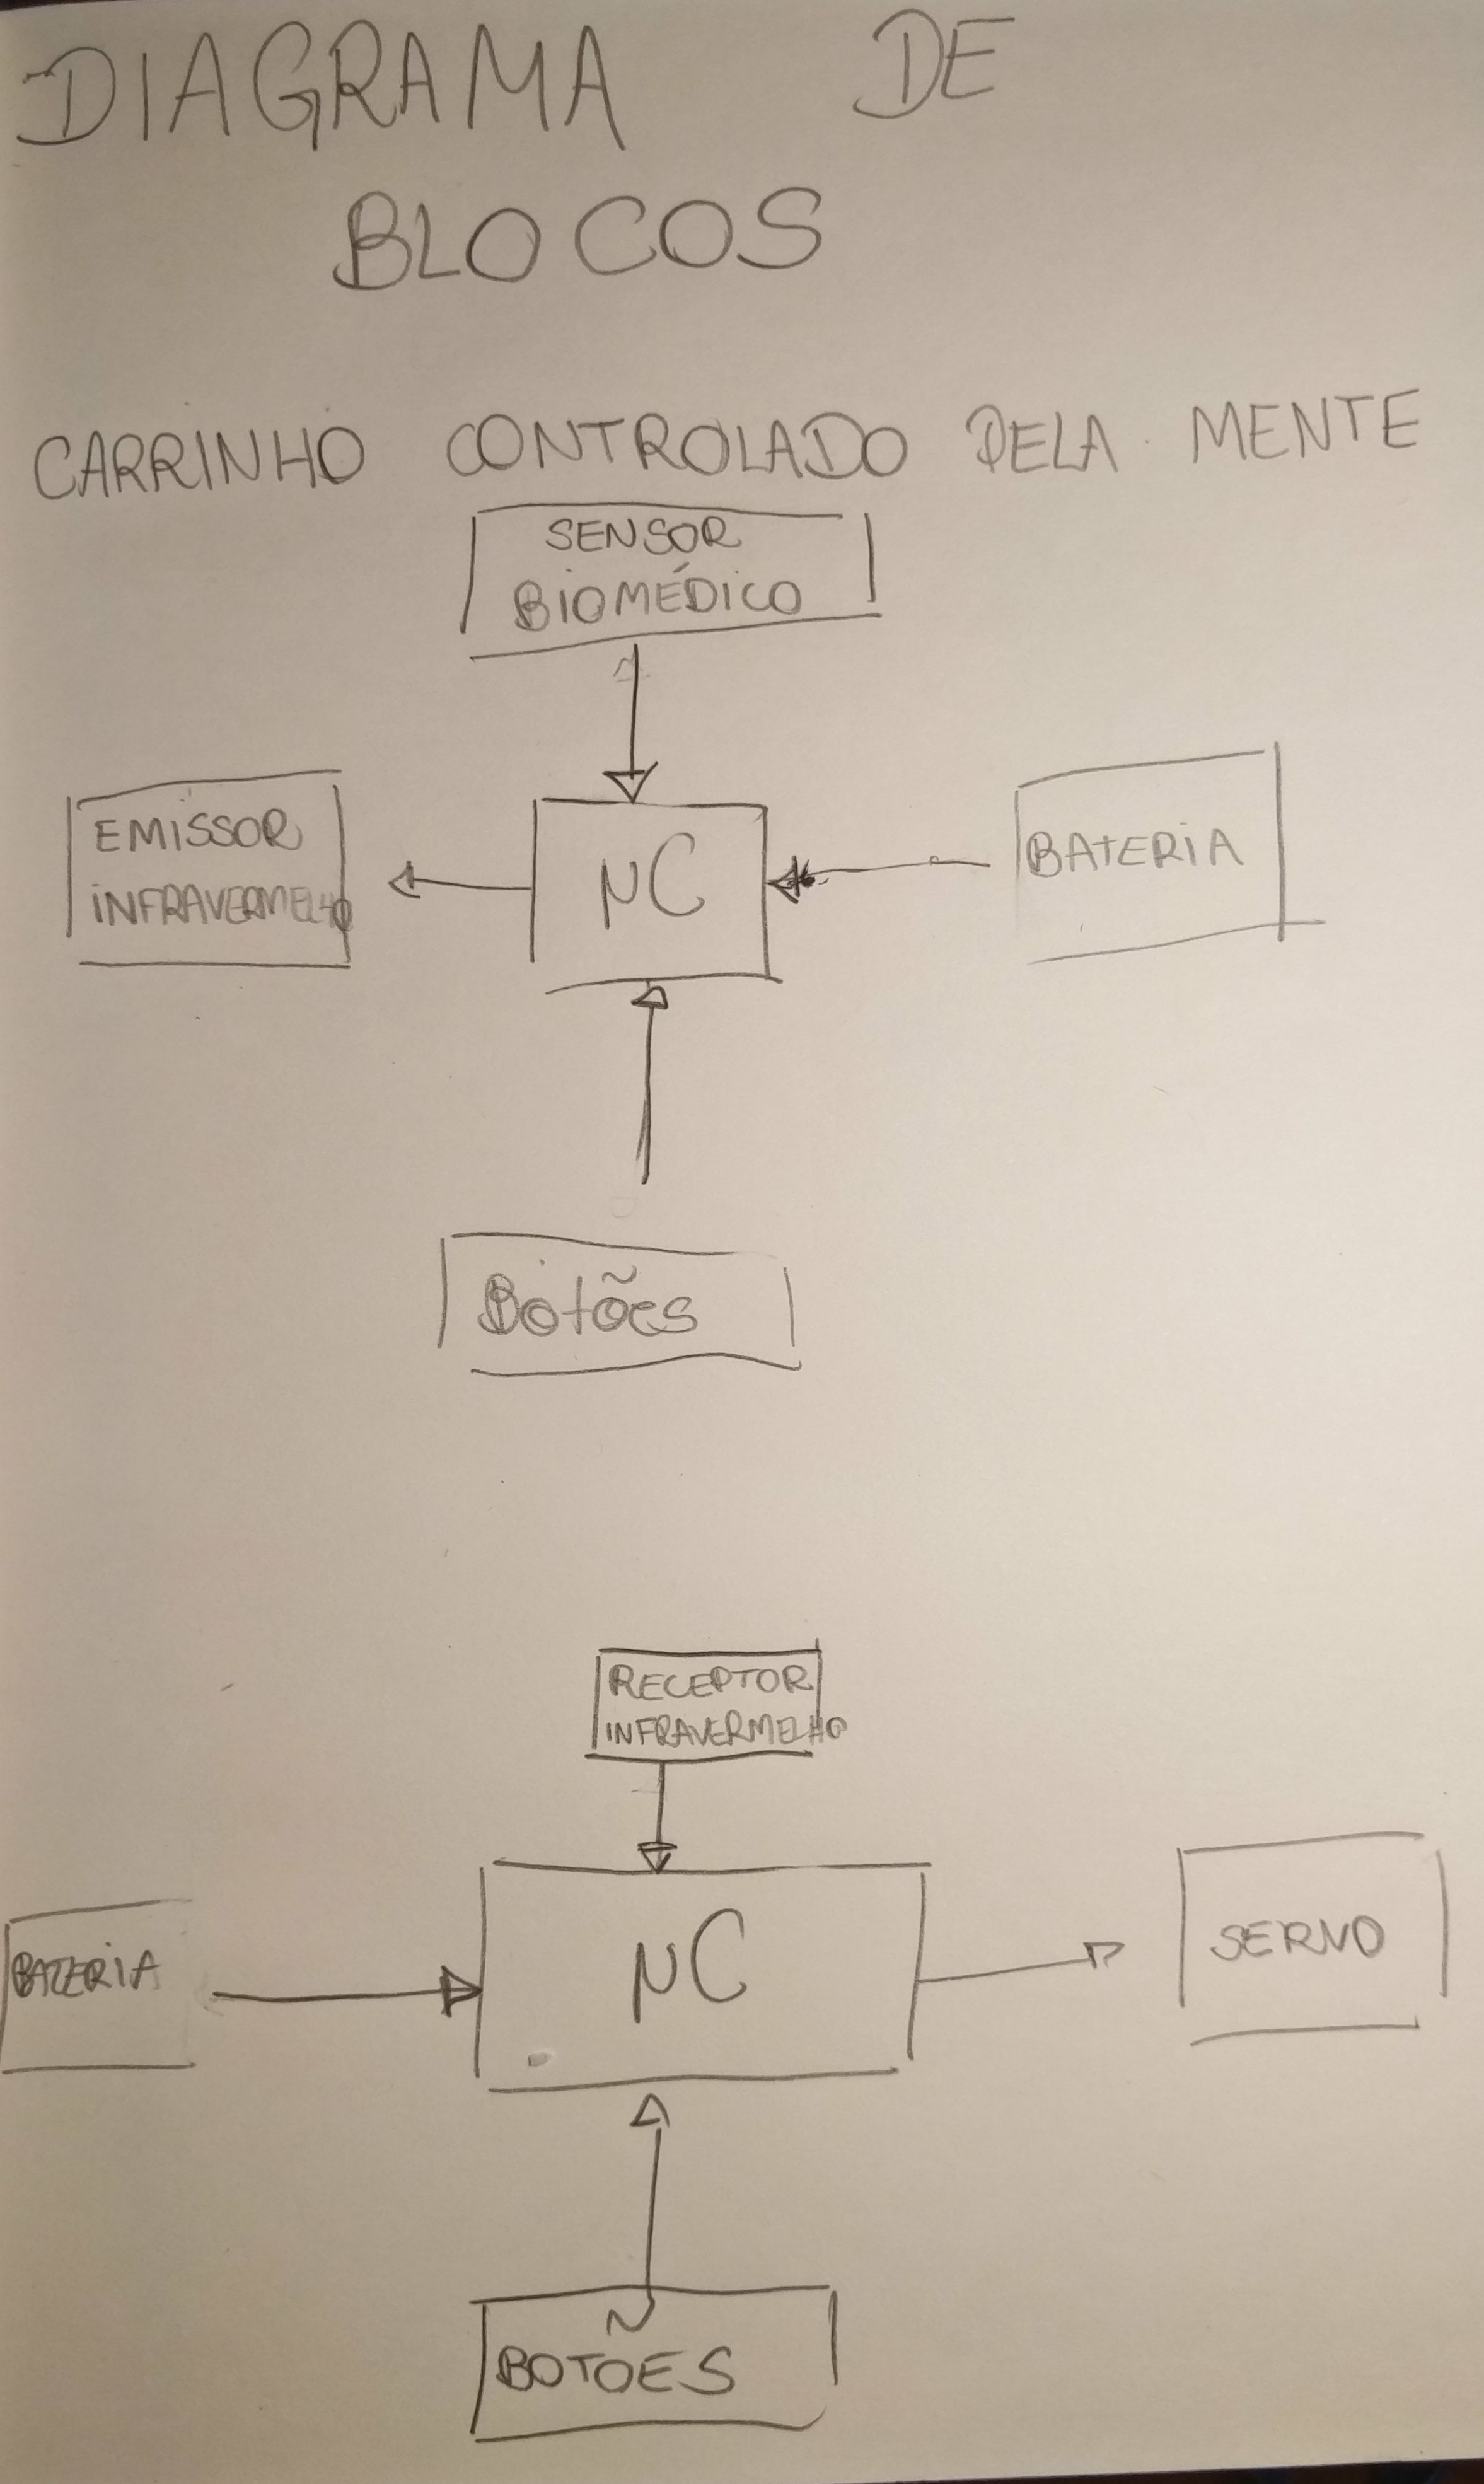
\includegraphics[width=0.7\textwidth]{fig2.jpg}
	\caption{Diagrama de blocos.}
\end{figure}

\raggedright
\part{3} \componentes
Esse projeto é dividido em duas partes, um pequeno carrinho simples e um embarcado que o controla. Os movimentos vão ser feitos através do sinal de sensores neurológicos para instruções muito simples, e serão convertidos em sinais eletromagnéticos. Esses sinais vão ser recebidos pelo carrinho para que o movimento seja executado.

Existem duas tecnologias principais nesse projeto, a requisição e tratamento de dados a partir de sensores neurológicos e o envio e recebimento dos sinais através de ondas eletromagnéticas.

\raggedright
\part{4} \gargalos

\RaggedRight
Como no primeiro projeto, por envolver sensores com sinais complexos, o recebimento e tratamento dos sinais gerados é o principal gargalo do projeto, ainda mais se tratando de sinais neurológicos. O envio e recebimento do sinal para o carrinho também é um gargalo do projeto, pois o emissor e o receptor devem estar pareados para o sinal funcionar.


\bibliography{ref}{}
\bibliographystyle{plain}
\end{document}